\chapter{Binding of Inositol Stereoisomers to Model Peptides}

The contents of this section were adapted from an article published in the \emph{Journal of Physical Chemistry}.
\\
\\
\emph{Reference}:
Li, G., Rauscher, S., Baud, S., Pom\`{e}s, R. (2012). Binding of Inositol Stereoisomers To Model Amyloidogenic Peptides. Journal of Physical Chemistry B, 116(3), 1111–1119.
\\
\\
\emph{Contributions}:
Grace Li conducted the research and wrote the section. R\'{e}gis Pom\`{e}s provided editorial input and guidance.

\newpage

\section{Summary}
The self-aggregation of proteins into amyloid fibrils is a pathological hallmark of numerous incurable diseases such as Alzheimer's disease. \textit{Scyllo-}-inositol is a stereochemistry-dependent  \textit{in vitro}  inhibitor of amyloid formation. As the first step to elucidate its mechanism of action, we present molecular dynamics simulations of \textit{scyllo-}inositol and its inactive stereoisomer, \textit{chiro-}inositol, with simple peptide models, alanine dipeptide (ADP) and $(Gly-Ala)_4$. We characterize molecular interactions and compute equilibrium binding constants between inositol and ADP as well as, successively, monomers, amorphous aggregates, and fibril-like \bsheet\ aggregates of $(Gly-Ala)_4$.\cite{Balbach:2000p49}
Inositol interacts weakly with all peptide systems considered, with mM to M affinities, and displaces the conformational equilibria of ADP but not of the $(Gly-Ala)_4$ systems. However, \textit{scyllo-} and \textit{chiro-}inositol adopt different binding modes on the surface of \bsheet\ aggregates. These results suggest that inositol does not inhibit amyloid formation by breaking up preformed aggregates, but rather by binding to the surface of pre-fibrillar aggregates.

\section{Introduction}
Amyloid fibrils formed by various peptides and proteins are known to be associated with neurodegenerative diseases, type II diabetes, and prion-related disorders.\cite{Chiti:2006p20} In particular, amyloid fibrils of \abeta\ peptides are found in the extracellular deposits of neuronal plaques and are thought to be central to the pathogenesis of Alzheimer's Disease (AD),\cite{Chiti:2006p20,Hardy:2002p27} a common and incurable neurodegenerative disease causing dementia and eventual death. 

In recent years, amyloid fibril formation was discovered to be a common phenomenon among many proteins in vitro; that is, under certain and denaturing conditions, proteins can self-aggregate to form amyloid fibrils.\cite{Chiti:2006p20} When viewed with negatively-stained transmission electron microscopy, amyloid fibrils appear as elongated, rope-like structures that are often 100 nm in length.\cite{Chiti:2006p20} The core structure of all amyloid fibrils is the cross-$\beta$-sheet.\cite{Chiti:2006p20,Serpell:2000p39} At the molecular level, NMR\cite{Balbach:2000p49,Petkova:2006p48} and X-ray crystallography\cite{Sawaya:2007p11} studies have revealed that the cross-$\beta$-structure is comprised of extended polypeptides organized in highly-ordered, in-register \bsheets. Although amyloid fibrils are a pathological hallmark of amyloid-based diseases, smaller nonfibrillar oligomers as little as three or four peptides in size have been demonstrated to display higher cytoxicity than mature fibrils.\cite{Gong:2003p22,Bitan:2003p10,Caughey:2009p5,Keshet:2010p61,Kitamura:2010p6,Lambert:1998p60,Selkoe:2008p16}

An important strategy to finding a cure to AD and other amyloid diseases is to derive new therapeutic candidates through the rational design of effective small-molecule inhibitors of amyloid formation. In recent years, a number of small molecules capable of preventing aggregation and/or fibril formation have been discovered and have emerged as potential therapeutic approaches for protein misfolding diseases.\cite{Frid:2007p65,Hawkes:2009p9,LeVine:2009p38,Necula:2007p42,ScherzerAttali:2010p63,Sood:2009p14} Interestingly, many of these small molecules share common chemical structural features, such as aromaticity and the presence of multiple hydrogen-bonding groups.\cite{Ehrnhoefer:2008p8,Liu:2009p18,Liu:2005p7,Porat:2006p33} However, the molecular basis of the structure-activity relationship of these small molecules is not understood, thus hindering drug development efforts for amyloid-based diseases.

Recently, one such small molecule, \textit{scyllo-}inositol, has shown promise as a therapeutic for AD.\cite{McLaurin:2006p29,McLaurin:2000p64} \textit{Scyllo-}-inositol is one of nine stereoisomers that belongs to a class of cyclic polyols called cyclohexanehexols. Four stereoisomers, \textit{myo-}, \textit{epi-}, \textit{scyllo-} and \textit{chiro-}inositol (Figure~\ref{fig:figure1}) are physiologically active.\cite{Fisher:2002p62} \textit{Myo-}inositol, the most abundant stereoisomer, plays an important role in signal transduction as precursor of phospholipid headgroups: once phosphorylated, \textit{myo-}inositol phosphatides act as second messengers in intracellular signal transduction pathways.\cite{Fisher:2002p62} Importantly for its therapeutic potential, inositol readily crosses the blood-brain barrier. \textit{Myo-} and \textit{scyllo-}inositol are found in tissues of the human central nervous system (CNS), with approximate concentrations of 5 mM and 0.1 to 0.5 mM, respectively.\cite{Michaelis:1993p89} Accordingly, they are also important osmolytes in the CNS, where alterations in their concentration have been associated with neuropathological conditions.\cite{Fisher:2002p62,Michell:2008p4}
 
\begin{figure}[htbp]
  \centering
  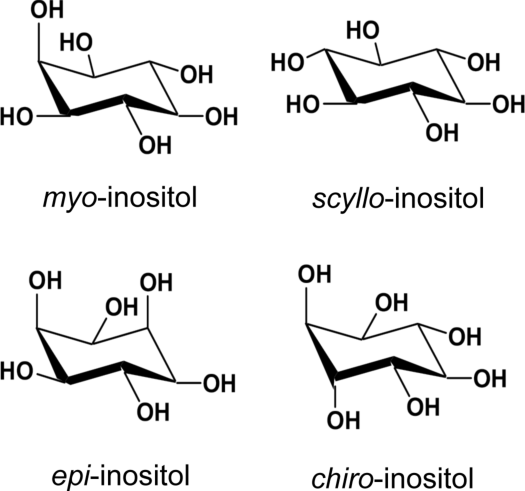
\includegraphics[width=3.25in]{figures/results1/GA4_paper_figures_submitted-1}
  \caption[Inositol stereoisomers most commonly found in nature.]
   {Inositol stereoisomers most commonly found in nature. Stick figures of the stereoisomers were drawn using the ChemDraw software.}
   \label{fig:figure1}
\end{figure}

In vitro, inositol stereoisomers stabilize nonfibrillar $\beta$-structure and prevent the formation of amyloid fibrils in a stereochemistry-dependent manner: \textit{scyllo-}, \textit{epi-} and \textit{myo-}inositol inhibit \abeta\ fibril formation, but not \textit{chiro-}inositol.\cite{McLaurin:2000p64,McLaurin:1998p176,Nitz:2008p13,Sun:2008p12,Townsend:2006p44} Moreover, \textit{scyllo-}inositol was also demonstrated to be the most effective stereosiomer in preventing and reversing AD-like symptoms in transgenic mice while reducing their brain plaque load.\cite{McLaurin:2006p29} Despite this progress, the molecular basis of amyloid inhibition by inositol is not understood. \textit{In vitro} studies suggest that inositol stereoisomers affects aggregation through direct interaction with \abeta\ peptides.\cite{McLaurin:1998p176,McLaurin:2000p64,Nitz:2008p13,Sun:2008p12} However, it is not known whether inositol acts on monomeric peptides, non-fibrillar oligomers, or fibrillar aggregates.

Some small molecule inhibitors, including the osmolytes glycerol and trimethylamine N-oxide (TMAO), are known to interfere with \textit{in vitro} aggregation of amyloidogenic peptides with different sequences,\cite{Scaramozzino:2006p69,Yang:1999p77,McLaurin:2000p76,Ehrnhoefer:2008p8,Dasilva:2010p25,Bieschke:2010p32} suggesting that generic interactions common to all amyloid-forming peptides and proteins may play a role in the inhibition of amyloid formation. Indeed, small organic osmolytes are hypothesized to modulate protein folding equilibria by interacting with the peptidic backbone, the chemical group common to all polypeptides.\cite{Street:2006p21,Hu:2010p46,Auton:2008p28} Accordingly, the role of backbone solvation in the modulation of protein folding\cite{Rose:2006p35,Auton:2008p28} and aggregation equilibria has recently been highlighted.\cite{Rauscher:2006p43} Furthermore, several studies have suggested that N-methylation of the backbone of amyloidogenic peptides can abolish the formation of amyloid fibrils by preventing intermolecular backbone hydrogen bonding.\cite{Takeda:2010p52,Soto:2007p171}

Experimental efforts to characterize the molecular interactions of small molecules with amyloid oligomers and fibrils are often impeded due to the non-crystalline, transient, and disordered nature of the aggregates involved. By contrast, molecular simulations are well-suited for studies of proteins involving disorder.\cite{Rauscher:2010p88} Although several molecular dynamics (MD) simulation studies have begun to examine the effect of small molecules on aggregation and fibril formation,\cite{Takeda:2010p34,Raman:2009p47,Lemkul:2010p23,Liu:2009p18} the role of backbone binding has not been considered systematically.

In this article, we present an MD simulation study of the interaction of inositol with simple model peptides to investigate its stereochemistry-dependent effect on amyloidogenic peptide aggregation and morphology. In a systematic approach, we first characterize the binding equilibria of \textit{myo-}, \textit{epi-}, \textit{scyllo-} and \textit{chiro-}inositol with alanine dipeptide, a model of the peptidic backbone. Next, to probe the stereochemistry-dependent effect of inositol binding on amyloid aggregation, we study the interaction of \textit{scyllo-} and \textit{chiro-}inositol, respectively active and inactive stereoisomers in \abeta\ amyloid inhibition, succcessively with monomer, disordered, and fibrillar aggregates of $(Gly-Ala)_4$ or \gafour. \gafour\ is one of the simplest and shortest amyloidogenic peptides that is known to adopt an extended \bsheet\ structure both synthetically,\cite{Rathore:2001p37} as a metallocopolymer,\cite{Vandermeulen:2006p15} and in nature, in crystalline domains of spider silks.\cite{Kenney:2002p45,Fossey:1991fk} The repetitiveness and simplicity of the peptide sequence allow us to achieve statistically-significant estimates of the binding equilibrium from conventional sampling methods while focusing on the effect of backbone interactions in polypeptide self-aggregation. 

\section{Methods}
\subsection{Simulation Parameters and Protocol}
Alanine dipeptide (ADP) was methylated at both the N- and C-terminii. The \gafour\ peptide was acetylated and amidated at the N- and C-termini, respectively. The peptides were built using PyMol\cite{Anonymous:2012p58} and modelled using the OPLS-AA/L force field\cite{Jorgensen:1996p19}. The extended OPLS-AA force field for carbohydrates\cite{Damm:1997p36} was used to model inositol stereoisomers and the TIP3P water model\cite{Jorgensen:1983p40} was used to represent the solvent. Versions 3.3.1 and 3.3.3 of the GROMACS software package\cite{VanDerSpoel:2005p56} were used to perform unrestrained all-atom MD simulations with the leap frog algorithm using an integration timestep of 2 femtoseconds. Unless otherwise noted, the following parameters were used for all simulations in this study. Electrostatic interactions were calculated using Particle Mesh Ewald (PME) summation with a grid size of 0.15 nm and a real-space cutoff of 1.45 nm.\cite{Essmann:1995p51} The Lennard-Jones potential was computed up to 1.3 nm and was switched to zero at 1.4 nm using the GROMACS switch function. The temperature and pressure were controlled at 300 K and at 1 atm using the Berendsen thermostat and pressure coupling scheme, respectively.\cite{Berendsen:1984p26} Covalent bonds involving hydrogens were constrained using the SHAKE algorithm.\cite{Ryckaert:1977p30} All resultant simulation systems were first subjected to energy minimization and equilibration with isotropic pressure coupling. Replicas of every system were generated with different random seeds for the choice of initial velocities. A trajectory frame was written to disk every picosecond and all frames were used in the final data analysis. Additional details of simulation setup and total sampling time for all systems performed in this study are listed in Table~\ref{tab:simulations}.
	
	% TODO Change the first column to be left-justified and resized ... HOW?
  \begin{table}\footnotesize
    \begin{center}
    \vspace{10pt}
    \label{tab:simulations}
      \begin{tabular}{| p{2.5cm} | *{7}{p{1.25cm}|}}
        \hline
        System & $N_{peptides}$ & $N_{inositol}$ & $c_{peptide}$ (mM) & $c_{Inositol}$ (mM) & $N_{replicas}$ & Time per replica ($\mu$s) & Total time ($\mu$s) \\
        \hline
        \hline
        alanine dipeptide & 1 & 0 & 61.5 & 0 & 5 & 0.1 & 0.5\\
        with \textit{myo-}, \textit{epi-}, \textit{chiro-} or \textit{scyllo}-inositol & 1 & 4 & 61.5 & 246 & 5 & 0.1 & 0.5 \\
        \hline
        \gafour\ monomer & 1 & 0 & 61.5 & 0 & 1117 & 0.005 & 5.585 \\
        with \textit{chiro-} or \textit{scyllo-}inositol & 1 & 2 & 61.5 & 123 & 1117 & 0.005 & 5.585 \\
        \hline
        \gafour\ disordered aggregate (preformed) & 4 & 0 & 246 & 0 & 5 & 0.1 & 0.5 \\
        with \textit{chiro-} or \textit{scyllo-}inositol & 4 & 2 & 246 & 123 & 5 & 0.08 & 0.4 \\
        \hline
        \gafour\ disordered aggregate (dispersed) & 4 & 0 & 246 & 0 & 5 & 0.1 & 0.5 \\
        with \textit{scyllo-} & 4 & 2 & 246 & 123 & 4 & 0.08 & 0.32 \\
        with \textit{chiro-} & 4 & 2 & 246 & 123 & 3 & 0.08 & 0.24 \\
        \hline
        \gafour\ fibrillar aggregate & 16 & 0 & 437 & 0 & 3 & 0.1 & 0.3 \\
        with \textit{chiro-} or \textit{scyllo-}inositol & 16 & 4 & 437 & 109 & 3 & 0.1 & 0.3 \\
        \hline
      \end{tabular}
      \caption{Summary of simulation systems.}
    \end{center}
  \end{table}

Five initial starting conformations of ADP were obtained by taking a frame every 20 ns from a 100-ns-long simulation of ADP in water. Sets of five independent simulations were carried out successively in the presence of \textit{myo-}, \textit{epi-}, \textit{chiro-} and \textit{scyllo-}inositol. The initial conformations of monomeric \gafour\ were taken from an ensemble of monomeric structures generated in water at 296 K by simulated tempering distributed replica sampling (STDR) from a previous study.\cite{Nikolic:2011p57} STDR is a generalized-ensemble simulation method developed in our laboratory, which allows each replica in the simulation to undergo a random walk in temperature to enhance conformational sampling.\cite{Rodinger:2006p78} The STDR algorithm and implementation are described elsewhere.\cite{Rauscher:2009p41} A representative set of 1117 structures were chosen from the STDR ensemble at 296 K such that the end-to-end distance probability distribution of this selected subset is similar to the distribution of the entire STDR ensemble of structures (about 12,000 structures in total). These conformations were then used as starting points for simulations at T = 300 K in the presence of two molecules of either \textit{scyllo-} or \textit{chiro-}inositol. A total of 5 $\mu$s of simulation time was generated for the monomeric systems with either \textit{scyllo-} or \textit{chiro-}inositol (Table~\ref{tab:simulations}). The initial peptide conformations of disordered oligomeric systems were either dispersed monomers drawn from the STDR ensemble at 296K or a preformed \bsheet\ oligomer of \gafour\ composed of four peptides.

The \gafour\ peptide in the extended conformation was constructed using PyMol and was used to create the fibril-like \bsheet\ model. An eight-stranded antiparallel \bsheet\ was constructed by first creating an antiparallel dimer of \gafour. The principal axis of the dimer was then aligned with the x-dimension of the box and translated along the y-axis to form a single 8-stranded \bsheet. Two of these 8-stranded sheets were stacked in parallel in a ``face-to-back" manner (with all Ala methyl groups facing up in the z direction) and placed in the simulation box such that the first strand at the edge of the \bsheets\ was hydrogen-bonded in-register to the nearest periodic image of the eighth strand. The fibril-like systems were first subjected to energy minimization and a 500 ps equilibration stage. Production simulations were performed in the NVT ensemble with final box dimensions of 4 nm x 3.8 nm x 4 nm. Three independent simulations of the \gafour\ fibril-like systems were performed for 100 ns each, successively in the presence and absence of \textit{scyllo-} and \textit{chiro-}inositol (see Table~\ref{tab:simulations}).

\subsection{Analysis Protocol}
The DSSP geometry criteria\cite{Kabsch:1983p31} were used to determine the presence of a hydrogen bond: (1) the distance between donor (D) and acceptor (A) atoms is less than 0.35 nm; (2) the distance between the hydrogen and A is less than 0.25 nm; and (3) the angle formed by D-H-A is greater than 120\mathdeg. Nonpolar contacts between inositol and peptide were defined by a separation between the center of mass of inositol and the C$_{\beta}$ atom of alanine less than 0.45 nm. The same cut-off was used to compute protein-protein nonpolar contacts between C$_{\beta}$ atoms. 

All of the dissociation constants for inositol were calculated based on the presence of intermolecular contacts as defined above. Then, assuming that the binding equilibrium of inositol is
	
% Equations used in the KLVFFAE paper                                                                                                                  
\begin{equation}
  \left[ Protein\cdot Inositol \right] 
  \rightleftharpoons 
  \left[ Protein \right]+\left[ Inositol \right]
\end{equation}
  
the dissociation constant is the equilibrium constant of this reaction and is given by 

\begin{equation}
  K_{d} = f_{ub}\frac{\left[ Protein \right]\left[ Inositol \right]}{\left[Protein \cdot Inositol\right]},
\end{equation}
 
where $f_{ub}$ is the fraction of unbound over bound peptide states.

The DSSP algorithm was used for the analysis of secondary structure of the disordered oligomer with N- and C-termini of the peptides excluded. The end-to-end distance for a \gafour\ peptide was calculated as the distance between C$_\alpha$ atoms of the N and C-terminus of the peptide. The spatial probability density of inositol is the average spatial occupancy of the atoms of inositol and was computed using the VolMap tool from the Visual Molecular Dynamics (VMD) software package. %XXX {humphrey, 1996 #143} 
The planar angle between inositol and the fibrillar model of \gafour\ was computed using the g\_sgangle program from GROMACS analysis tools. All planar angles were corrected to a value between 0\mathdeg\ and 90\mathdeg, using the rule $\alpha = f(\theta) = 180 - \theta$, if $\theta > 90$\mathdeg, otherwise, $f(\theta) = \theta$. The probability distribution of the planar angles, $P(\alpha)$, was determined for inositol molecules with atoms within 0.25 $nm$ of the fibril. Average nonpolar and hydrogen bonding contacts in disordered aggregates were computed using the last 70 $ns$ of each trajectory. Error bars were determined by computing the standard deviation of the averages obtained from trajectories of independent replicas. Block averaging was used whenever a single trajectory was available.

\section{Results}
Inositol was found to bind weakly and reversibly to all the peptidic systems considered in our simulations, allowing us to characterize binding equilibria from unbiased sampling.

% This is a table with footnotes and with the footnote rule removed
% It uses the minipage and I had to tweak the width of the page so that center can 
% properly align the table in the middle of the page.
\begin{table}\footnotesize
  \vspace{10pt}
  \label{tab:binding_constants}
  \begin{minipage}{15cm}
    \renewcommand{\thefootnote}{\thempfootnote}
    \renewcommand{\footnoterule}{}
    % \centering
      \begin{center}
    \begin{tabular}{| l | *{5}{ c |}}
       \hline
         System & \textit{Scyllo-}\footnote{Each dissociation constant is in units of mM. The standard error is shown within parentheses.} & \textit{Chiro-} \footnotemark[\value{mpfootnote}] & N$_{groups,ADP}$/N$_{groups}$ & \textit{Scyllo-} \footnote{K$_d$ in units of $mM$, estimated by scaling the K$_d$ of ADP by the ratio of the number of \\ peptide groups in ADP to the \gafour\ system} & \textit{Chiro-}\footnotemark[\value{mpfootnote}]\\
         \hline
         \hline
         alanine dipeptide & 1100 (100) & 1000 (100) & 1.00 & 1100 & 1000 \\ 
         \gafour\ monomer & 376 (10) & 362 (16) & 0.25 & 275 & 250 \\ 
         \gafour\ preformed & 85 (12) & 89 (8) & 0.06 & 69 & 63 \\ 
         \gafour\ dispersed & 87 (21) & 86 (10) & 0.06 & 69 & 63 \\ 
         \gafour\ fibrillar & 51 (3) & 36 (15) & 0.02 & 17 & 16 \\
         \hline
     \end{tabular}   
  \end{center}
  \end{minipage}
  \centering
  \caption{Summary of equilibrium dissociation constants (K$_d$) for each system in the study.}
  \end{table}


\subsection{Alanine dipeptide}
Inositol stereoisomers bound weakly and reversibly to alanine dipeptide with a molar \KD. A list of computed dissociation constants for each stereoisomer is shown in Table~\ref{tab:binding_constants}. Because all of the results for \textit{myo-} (1.0 $\pm$ 0.1 M), \textit{epi-} (1.2 $\pm$ 0.2 M), \textit{chiro-} (1.0 $\pm$ 0.1 M) and \textit{scyllo-}inositol (1.1 $\pm$ 0.1 M) were within error bars of one another, in this section we provide detailed descriptions and data only for \textit{scyllo-}inositol. A single molecule of \textit{scyllo-}inositol can bind the peptidic backbone in either monodentate or bidentate fashion, as defined by the number of hydrogen bonds between hydroxyl groups of inositol and peptide groups. At a concentration of 250 mM, \textit{scyllo-}inositol was bound in the monodentate and bidentate modes about 14 $\pm$ 1\% and 1.1 $\pm$ 0.1\% of the time, respectively. The dominant bidentate binding modes of \textit{scyllo-}inositol involved hydrogen bonds formed with the peptide main chain either in the mean plane of the inositol ring (Figure~\ref{fig:figure2}, panels I-III) or in a ``face-to-edge" fashion, where the mean plane of the inositol ring is perpendicular to the plane of the peptide groups (Figure~\ref{fig:figure2}A, panel IV).
	
\begin{figure}[htbp]
    \centering
    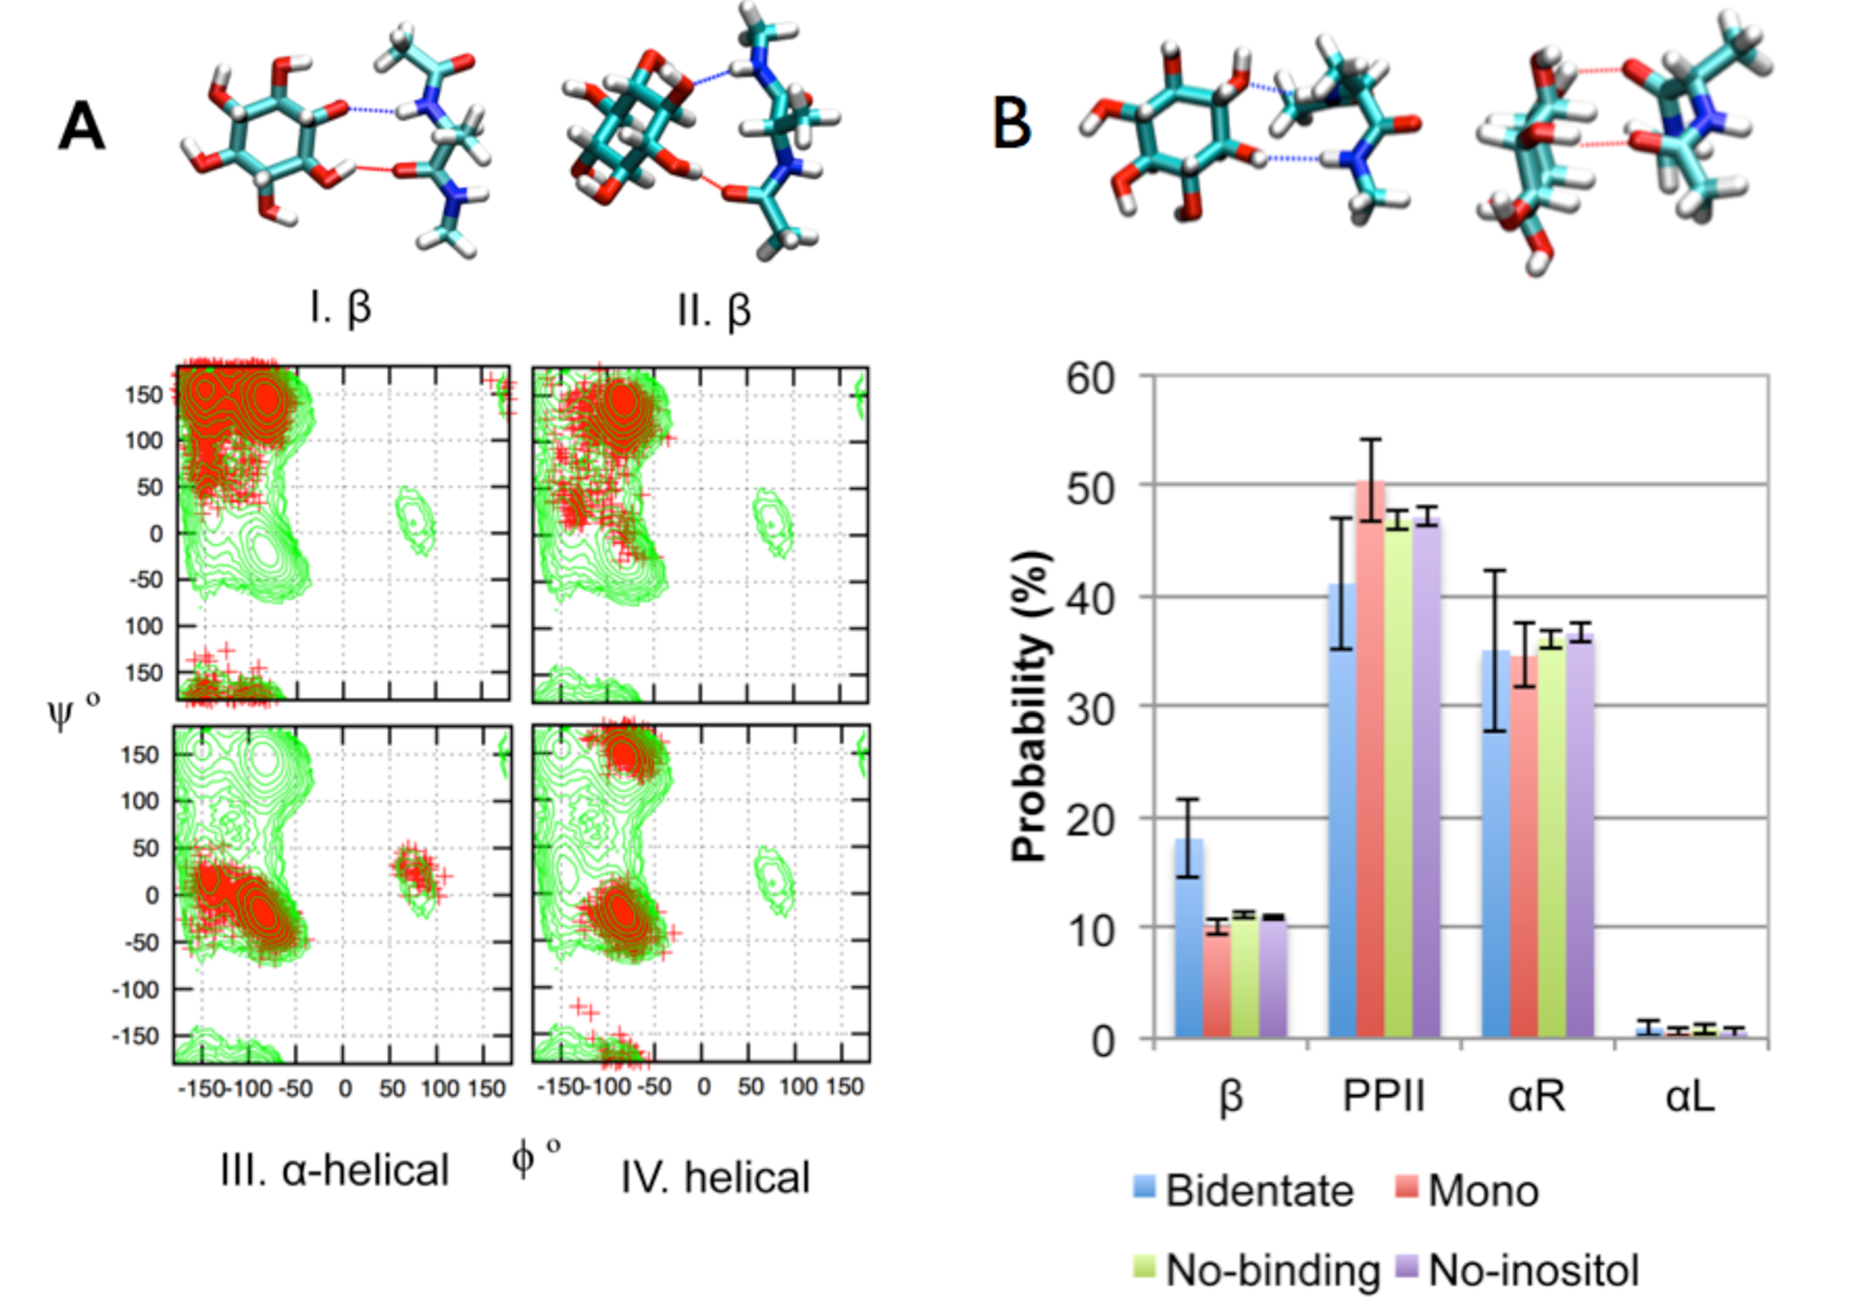
\includegraphics[width=6in]{figures/results1/GA4_paper_figures_submitted-2-rearranged}
    \caption[Binding of \textit{scyllo-}inositol to the backbone of alanine dipeptide.]
     {Binding of \textit{scyllo-}inositol to the backbone of alanine dipeptide. A) Main bidentate binding modes. Ramanchandran maps of the conformations of alanine dipeptide sampled in absence of inositol are shown as contours in green. ($\phi$,$\psi$) of alanine dipeptide conformers bound by inositol are shown on the map as red crosses. $\beta$-conformers (top panels) are bound by inositol through adjacent or non-adjacent (CO,NH) groups; Helical conformers (bottom panels) involve mostly (CO,CO) and (NH,NH) groups. B) Comparisons of the conformational equilibrium of alanine dipeptide for different inositol backbone-bound states.}
     \label{fig:figure2}
  \end{figure}
  
The Ramachandran map of ADP is characterized by four dominant basins representing the α-helical, polyproline II (PPII), and \bsheet\ conformations.\cite{Neale:2008p87} As shown in Figure~\ref{fig:figure2}A, bidentate-bound ADP adopts backbone dihedral angles that fall within the dominant basins on the ramachandran map, demonstrating that \textit{scyllo-}inositol is able to bind both helical and \bsheet\ conformations. Notably, the conformational equilibrium of ADP is shifted in favor of the $\beta$-conformer when \textit{scyllo-}inositol is bound to the peptide backbone in bidentate fashion (Figure~\ref{fig:figure2}B); in contrast, the relative populations of dominant conformers remained unchanged when inositol is unbound or bound in monodentate form. Taken together, our results show that although binding is weak, inositol may influence peptide conformations by binding to the peptidic backbone. In the next sections, we examine the binding of inositol to monomer and aggregates of a simple \bsheet\ forming peptide, \gafour.

\begin{figure}[htbp]
  \centering
  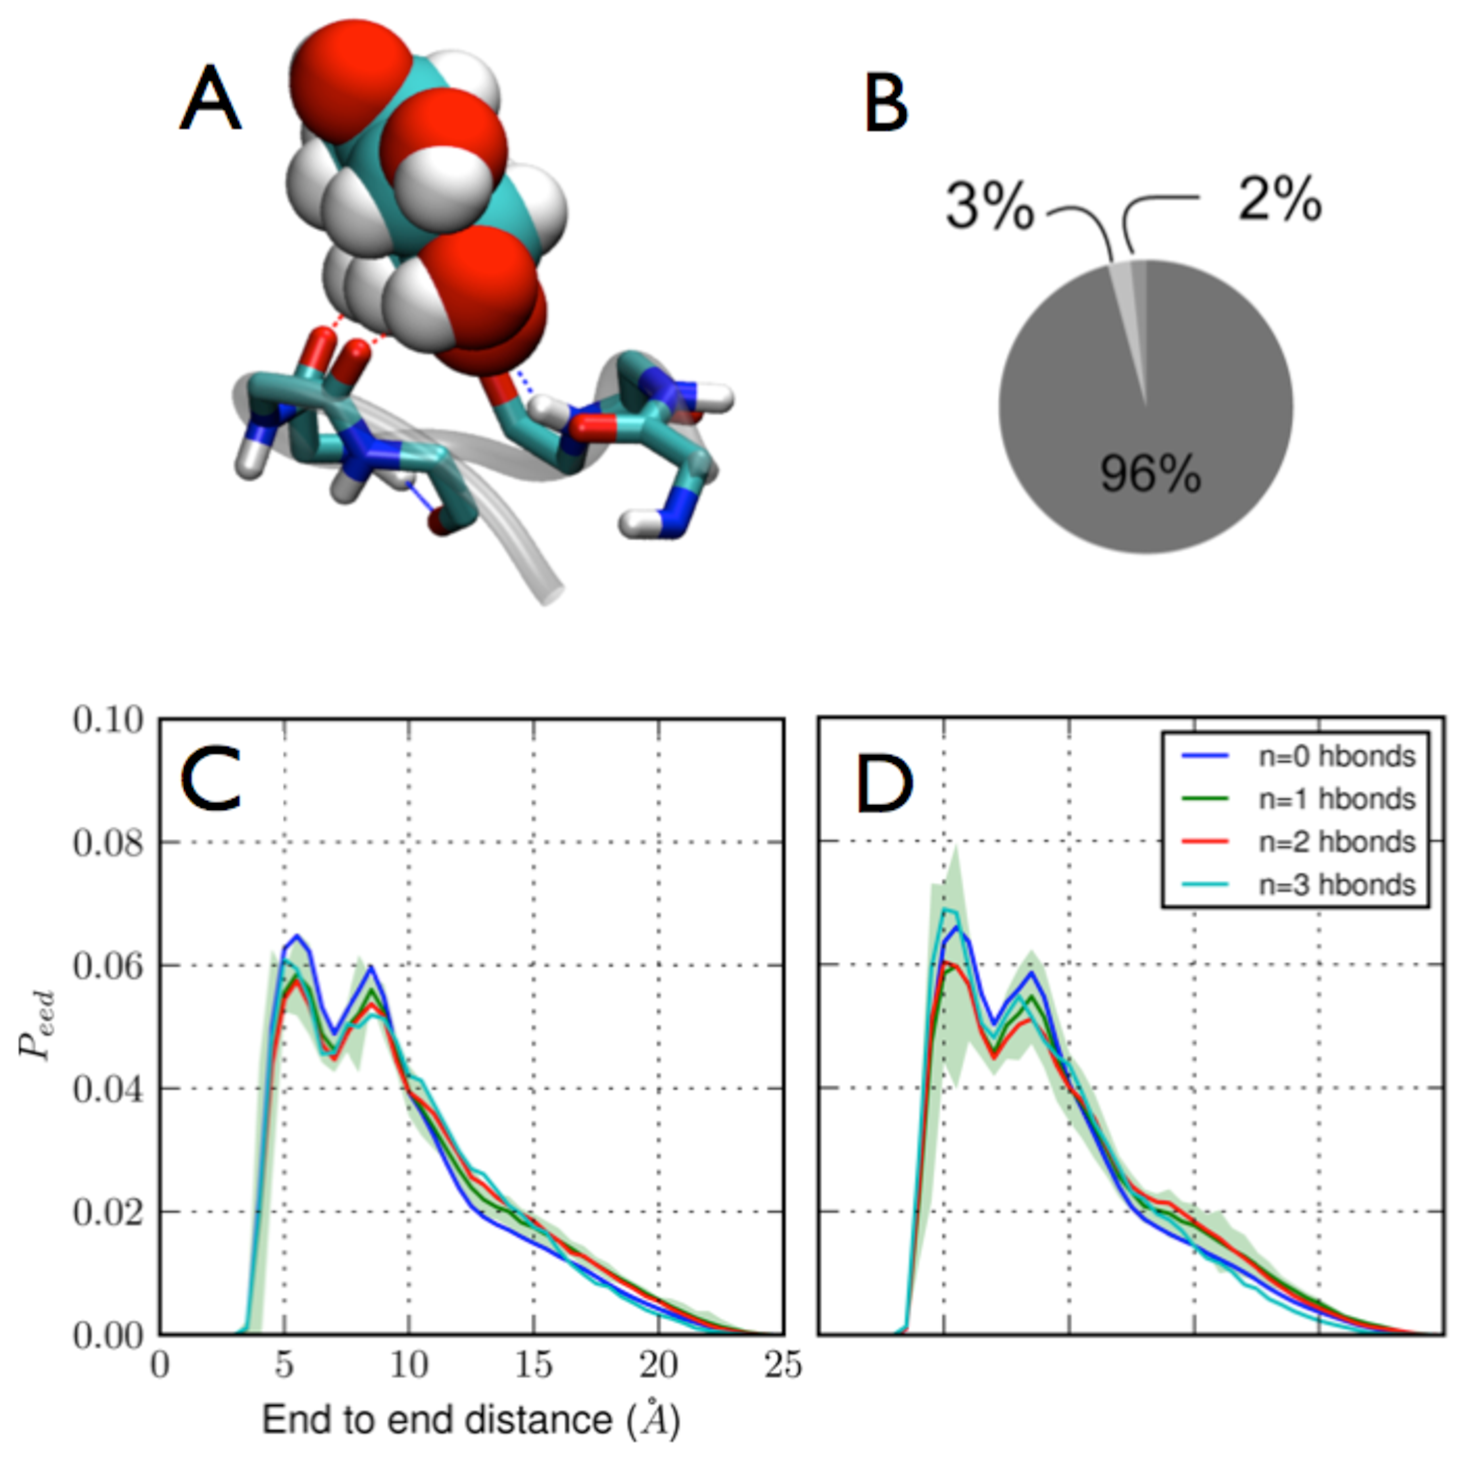
\includegraphics[width=5in]{figures/results1/GA4_paper_figures_submitted-3-rearranged}
  \caption[Binding of \textit{scyllo-}inositol to the monomer of (GA)$_4$.]{Binding of \textit{scyllo-}inositol to the monomer of (GA)$_4$. A) Representative snapshot of \textit{scyllo-}inositol forming three hydrogen bonds to a monomer of (GA)$_4$. B) Distribution of the fraction of bound \textit{scyllo-}inositol to polar and nonpolar groups of the monomer. C-D) Conformational equilibrium of (GA)$_4$ as measured by the peptide end-to-end distance distribution. The distributions are all within error bars of each other and are plotted separately by the number of hydrogen bonds for \textit{scyllo-} in C) and \textit{chiro-}inositol in D). For clarity, error is only shown for the Peed curve where $n$=1.}
   \label{fig:figure3}
\end{figure}

\subsection{\gafour\ peptide}
In this section, we characterize the binding modes and binding affinity of inositol systematically, first with a peptide monomer, and then with oligomeric and fibrillar aggregates of \gafour. Here we examine only the active and inactive stereoisomers \textit{scyllo-} and \textit{chiro-}inositol. A summary of the equilibrium binding constants computed for all \gafour\ systems is shown in Table~\ref{tab:binding_constants}.

\subsubsection{Monomer}
In its monomeric state in solution, \gafour\ is an intrinsically disordered peptide.\cite{Nikolic:2011p57} An example of \textit{scyllo-}inositol binding to a monomer is shown in Figure~\ref{fig:figure3}A. Similar to ADP, binding is weak: the computed dissociation constants were \KD$_{,chiro}$  $\approx$ 362 $\pm$ 16 mM and \KD$_{,scyllo}$  $\approx$ 376 $\pm$ 10 mM. Most bound states, 95\% for \textit{scyllo-}inositol and 94.4\% for \textit{chiro-}inositol, involved hydrogen bonds to the backbone (Figure~\ref{fig:figure3}B). At a concentration of 123 mM, inositol molecules formed a single hydrogen bond about 9\% of the time, whereas two or more hydrogen bonds were formed about 4 to 5\% of the time. In contrast, nonpolar contacts are less frequent and, alone, account for only 3\% of bound \textit{scyllo-} and \textit{chiro-}inositol (Figure~\ref{fig:figure3}B). In total, the peptide monomer is bound to at least one molecule of inositol approximately 25\% of the time, 23\% of the time with a inositol:peptide stoichiometry of 1:1 and only $\sim$2\% of the time with a 2:1 stoichiometry. Contrary to ADP, the presence of inositol did not have a significant effect on the conformational equilibrium of monomeric \gafour\ (Figure~\ref{fig:figure3}C-D).

\subsubsection{Disordered Oligomer}

\begin{figure}[htbp]
  \centering
  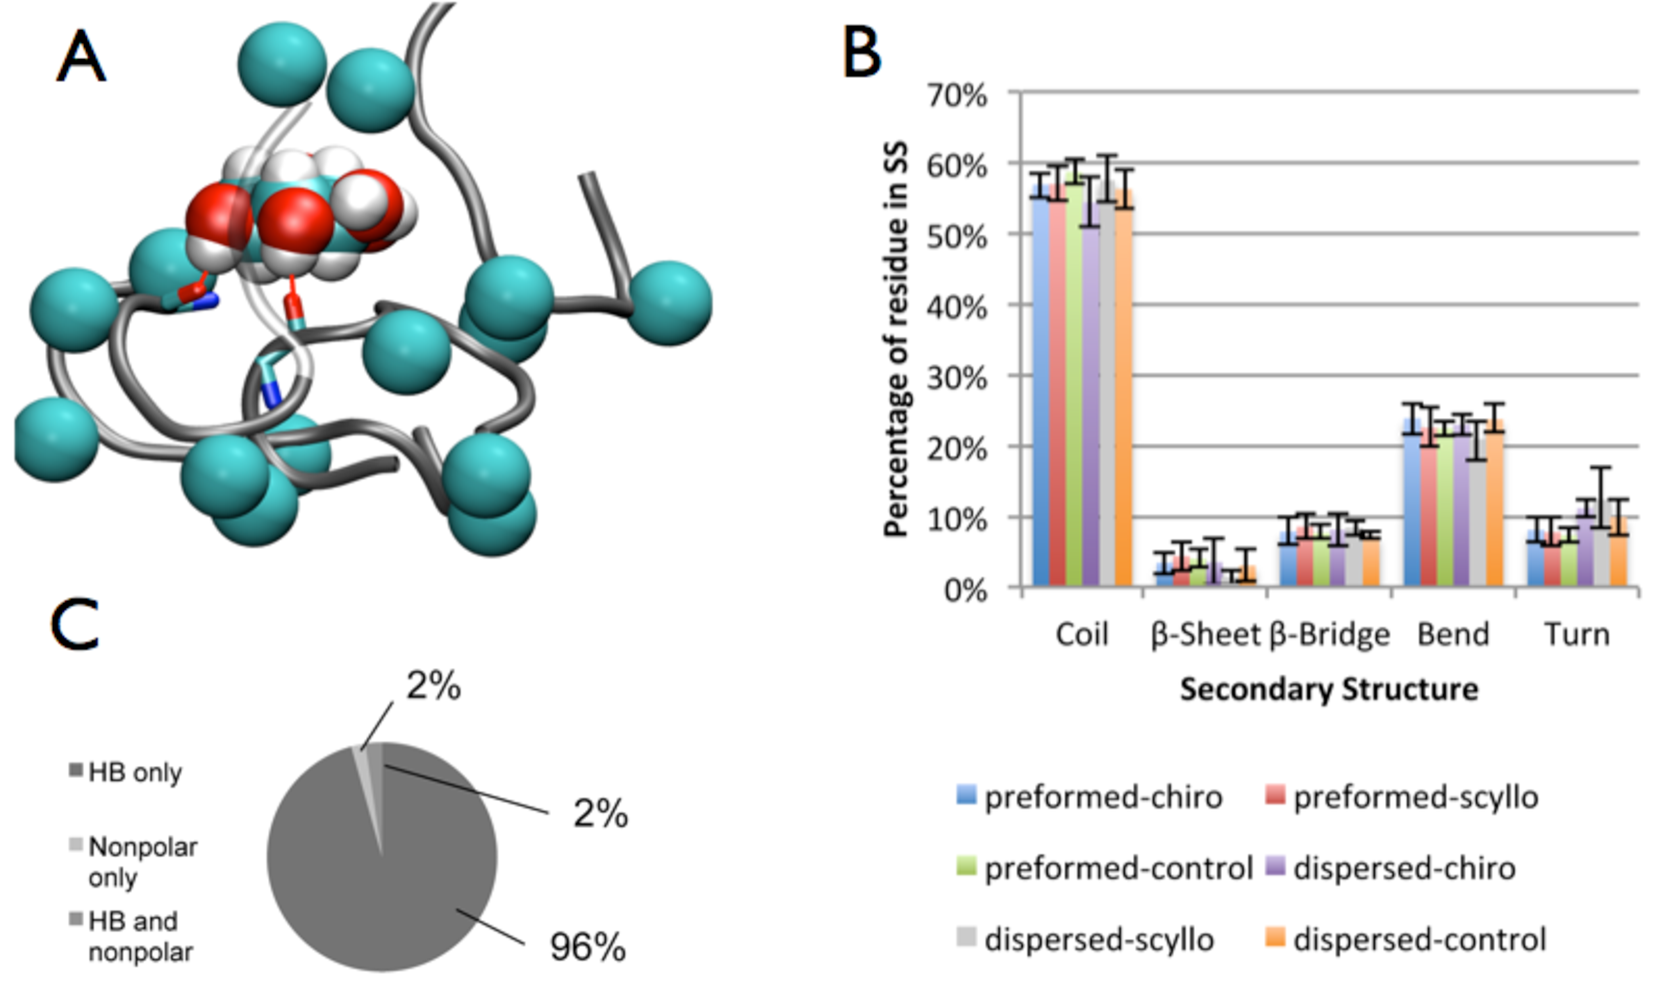
\includegraphics[width=6in]{figures/results1/GA4_paper_figures_submitted-4-rearranged}
  \caption[Binding of \textit{scyllo-}inositol to the disordered oligomer of \gafour.]{Binding of \textit{scyllo-}inositol to the disordered oligomer of \gafour. A) Snapshot of \textit{scyllo-}inositol simultaneously hydrogen bonding two peptides in a disordered \gafour\ aggregate. Hydrogen bonds to the backbone are drawn as red lines. B) Distribution of secondary structure content, as classified by the DSSP algorithm, for preformed and dispersed starting states of the oligomer. Hydrogen bonds to the backbone are drawn as red lines. C) Fraction of \textit{scyllo-}inositol interacting with the disordered oligomer via hydrogen bonds (HBs), nonpolar contacts, or both. The fractions for \textit{chiro-}inositol are similar (data not shown).}
   \label{fig:figure4}
\end{figure}

To probe whether inositol affects the structure and aggregation of small oligomers of \gafour\ in solution, we performed sets of simulations involving two distinct starting states of four \gafour\ peptides: (1) initially monodispersed peptides and (2) a preformed \bsheet\ aggregate. In the initially dispersed systems, the peptides rapidly aggregated to form a disordered oligomer (Figure~\ref{fig:figure4}A) in which the majority of the residues ($\sim$60\%) retained a coil conformation (Figure~\ref{fig:figure4}B). Similarly, systems initiated with a preformed 4-stranded \bsheet\ also evolved into a disordered oligomer over the course of the simulation. Only about 5\% and 10\% of the residues participated in a \bsheet\ or in a \bbridge, respectively (Figure~\ref{fig:figure4}B).
	
\begin{figure}[htbp]
  \centering
  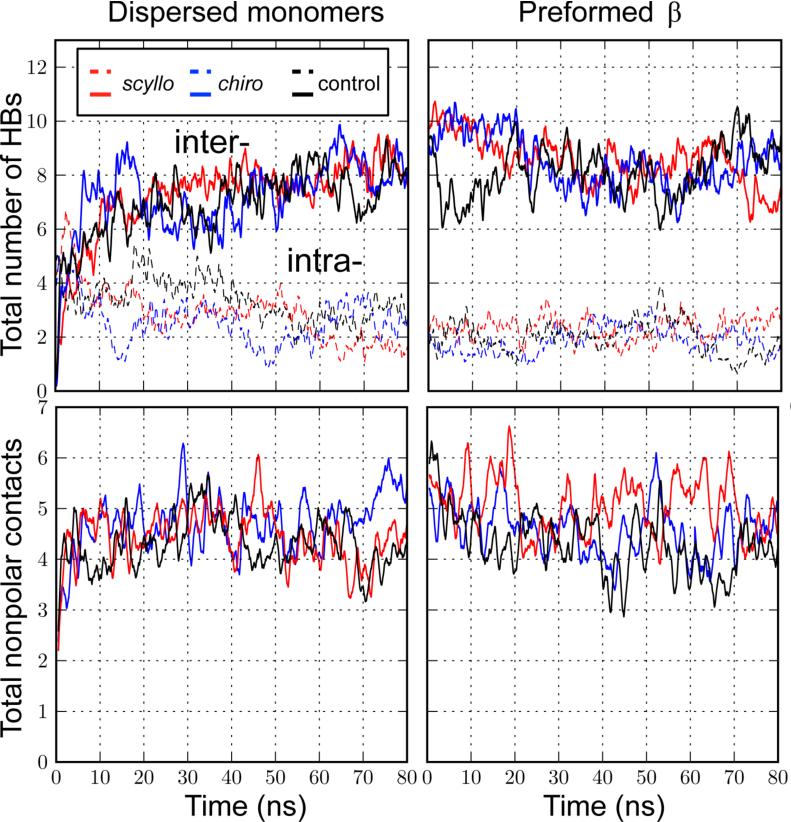
\includegraphics[width=4.5in]{figures/results1/GA4_paper_figures_submitted-5}
  \caption[Time evolution of peptide-peptide nonpolar and hydrogen bonding contacts in disordered aggregates in presence and absence of inositol (control).]{Time evolution of peptide-peptide nonpolar and hydrogen bonding contacts in disordered aggregates in presence and absence of inositol (control). Each curve is smoothed using a running average over a window with a length of 500 ps. Results for the dispersed monomer aggregates are shown on the left and the preformed $\beta$-sheet aggregates on the right. Top: the total number of inter- and intra-molecular hydrogen bonding contacts; Bottom: Number of intermolecular nonpolar contacts.}
   \label{fig:figure5}
\end{figure}
  
Despite different initial conditions and independently of the presence of inositol, all aggregates evolved to a similar morphology. The total number of peptide-peptide nonpolar and polar contacts formed within the oligomer converged to similar values for both the dispersed and preformed oligomers and did not change with time (Figure~\ref{fig:figure5}). As shown in Figure~\ref{fig:figure5} (top panels), the average total number of intermolecular hydrogen bonds ($\sim$8 $\pm$ 1) was consistently \bbridge\ higher than the number of intramolecular hydrogen bonds ($\sim$2.1 $\pm$ 0.3). On average, about 4.3 $\pm$ 0.4 nonpolar contacts were formed upon aggregation in the absence of inositol compared to 4.4 $\pm$ 0.5 contacts for \textit{scyllo-}, and 5.0 $\pm$ 0.4 for \textit{chiro-}inositol (data not shown for the preformed oligomer). When taken together, the above results show that the presence of \textit{scyllo-} and \textit{chiro-}inositol neither prevented aggregation nor disrupted the preformed oligomer.

Dissociation constants of about 80 mM to aggregates of type 1 and 2 were obtained for both \textit{scyllo-} and \textit{chiro-}inositol. The \KD\  calculated for each aggregate type is shown in Table~\ref{tab:binding_constants}. In the presence of multiple aggregated chains, a single molecule of inositol was found to cross-link multiple peptides by simultaneously hydrogen bonding to their backbones (Figure~\ref{fig:figure4}A). Similar to monomers, at a concentration of 123 mM, \textit{chiro-} and \textit{scyllo-}inositol were bound predominantly to the backbone: ~96\% of bound \textit{scyllo-}inositols formed only hydrogen bonding contacts ($\sim$94\% for \textit{chiro-}inositol), whereas 2\% (3\% for \textit{chiro-}inositol) were involved in nonpolar contacts only (Figure~\ref{fig:figure4}C).

\subsubsection{Fibril-like oligomer} % (fold)

\begin{figure}[htbp]
  \centering
  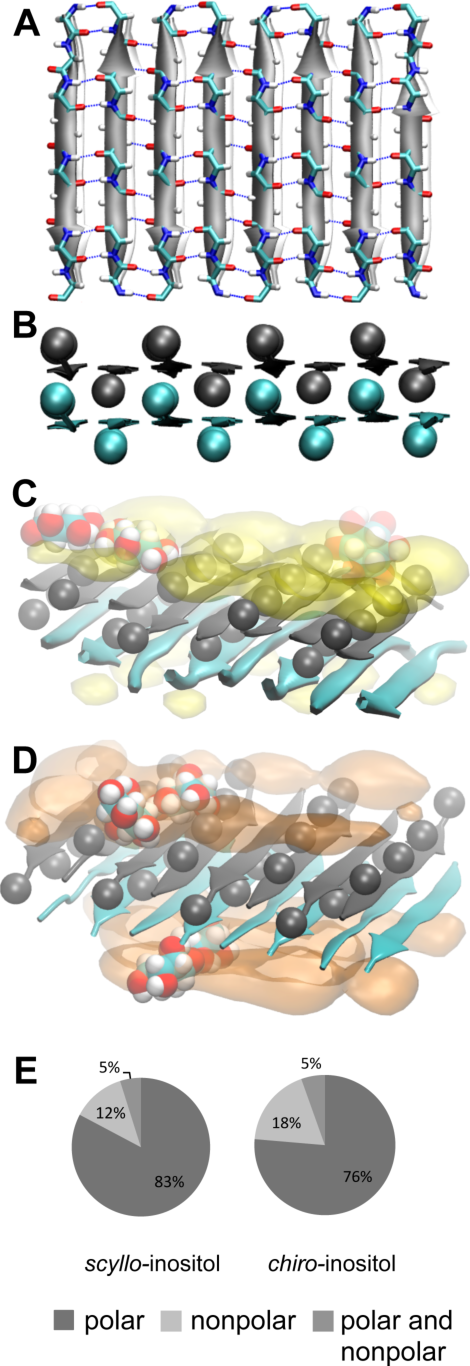
\includegraphics[scale=0.75]{figures/results1/GA4_paper_figures_submitted-6}
  \caption[Binding of \textit{scyllo-} and \textit{chiro-}inositol to the fibrillar aggregate of \gafour.]{Binding of \textit{scyllo-} and \textit{chiro-}inositol to the fibrillar aggregate of \gafour. Different views of the initial starting structure of the fibril-like model. Top and bottom sheets are colored in grey and in cyan, respectively. A top down view is depicted in A) showing the backside of the top \gafour\ sheet. A side view of the protofibril is shown in B). The spatial probability density of bound \textit{scyllo-}inositol (yellow) C) and \textit{chiro-}inositol (orange) D) are shown overlapping with the fibril. The density is shown at an occupancy isosurface value of 3\% for both stereoisomers. E) is the percentage of bound \textit{scyllo-} and \textit{chiro-}inositol to polar and nonpolar groups on the \bsheet.}
   \label{fig:figure6}
\end{figure}

In order to probe the binding modes of inositol with a fibril-like aggregate of \gafour, we constructed an ‘infinite \bsheet’, where the $\beta$-strands at the edge of an octameric \bsheet\ are hydrogen-bonded to each other’s nearest periodic image. A single unit of this periodic model consisted of a stack of two antiparallel and in-register \bsheets, with eight strands per sheet (Figure~\ref{fig:figure6}A,B). Although some of the hydrogen bonds defining the \bsheet\ structure occasionally broke, in the absence of inositol the protofibril remained approximately planar and aggregated as an infinite fibril throughout the simulation.

The spatial distribution of bound inositol molecules shows that both \textit{chiro-} and \textit{scyllo-}inositol bind at the surface of the fibril (Figures~\ref{fig:figure6}C, D). \textit{Chiro}- and \textit{scyllo-}inositol bound fibrillar aggregates of \gafour\ with a \KD\ of 36 $\pm$ 15 mM and 51 $\pm$ 3 mM, respectively. The apparent increase in affinity compared to amorphous aggregates can be attributed to the following reasons. First, the fibrillar aggregate presents a much larger effective surface area than both the monomer and the disordered oligomer (Figures~\ref{fig:figure6}C, D). Moreover, a larger fraction of the alanine side chains are completely solvent-exposed in the fibril-like aggregate, increasing the fraction of bound conformations involving only nonpolar contacts by nearly an order of magnitude, from 2\% in the disordered oligomer to 12\% for \textit{scyllo-} and 18\% for \textit{chiro-}inositol in the fibrillar aggregate in the presence of 109 mM of inositol (Figures~\ref{fig:figure3}B and \ref{fig:figure6}E). Accordingly, a higher fraction of \textit{scyllo-}inositol, 83 $\pm$ 1\%, versus 77 $\pm$ 1\% for \textit{chiro-}inositol, was found to form hydrogen bonds, where the 6\% drop in the hydrogen-bonded-only population of \textit{chiro-}inositol was compensated by a commensurate increase in the nonpolar-bound-only population of \textit{chiro-}inositol (Figure~\ref{fig:figure6}E).

\begin{figure}[htbp]
  \centering
  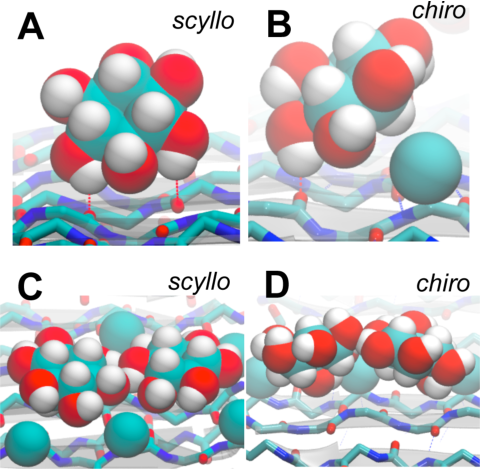
\includegraphics[width=3.2in]{figures/results1/GA4_paper_figures_submitted-7}
  \caption[Example snapshots of \textit{scyllo-} and \textit{chiro-}inositol binding to the fibril of \gafour.]{Example snapshots of \textit{scyllo-} and \textit{chiro-}inositol binding to the fibril of \gafour. Red and blue dashed lines denote hydrogen bonds. A-B) Example binding modes of \textit{scyllo-} and \textit{chiro-}inositol binding at an angle to the surface. C-D) Example binding modes of \textit{scyllo-} and \textit{chiro-}inositol binding face down on the sheet.}
   \label{fig:figure7}
\end{figure}

Thus, although \textit{chiro-} and \textit{scyllo-}inositol have similar binding constants, they have different binding modes to fibrillar aggregates, a feature not previously observed for the monomer and the disordered oligomer of \gafour. Both \textit{scyllo-} and \textit{chiro-}inositol form nonpolar contacts and backbone hydrogen bonds in poses where the mean plane of the inositol ring lies parallel, at an angle, or perpendicular to the plane of the fibril (Figure~\ref{fig:figure7}). Furthermore, two or more molecules of inositol may cluster together and bind at the surface of the sheet (Figures~\ref{fig:figure7}C,D). However, as shown in Figure~\ref{fig:figure8}A, \textit{scyllo-}inositol adopts specific binding orientations whereas \textit{chiro-}inositol does not: \textit{scyllo-} preferentially binds in either nearly flat ($\alpha = 20$\mathdeg) or upright ($\alpha = 65$\mathdeg) to the sheet, whereas \textit{chiro-}inositol does not have such a bimodal preference and binds the fibril at an average angle of $\alpha = 45$\mathdeg. This stereochemistry-modulated difference in binding specificity explains the somewhat higher fraction of nonpolar binding by \textit{chiro-}inositol (Figure~\ref{fig:figure6}E): \textit{chiro-} is more likely than \textit{scyllo-}inositol to bind at angles of $30$\mathdeg $< \alpha \leq 60$\mathdeg (Figure~\ref{fig:figure8}A), where 24\% of bound \textit{chiro-} (versus 16\% for \textit{scyllo-}inositol) is bound by nonpolar contacts only (Figure~\ref{fig:figure8}B). For $\alpha \leq 30$\mathdeg, the distributions of \textit{scyllo-} and \textit{chiro-}inositol bound to polar and nonpolar groups are similar (data not shown). Moreover, because \textit{chiro-}inositol has a partially-nonpolar edge whereas \textit{scyllo-}inositol does not, binding in the upright position also involves more nonpolar interactions for \textit{chiro-} than for \textit{scyllo-}inositol (Figure~\ref{fig:figure8}B). Finally, although inositol was observed to bind at the surface, binding did not change the morphology of the fibrillar aggregate.

\begin{figure}[htbp]
  \centering
  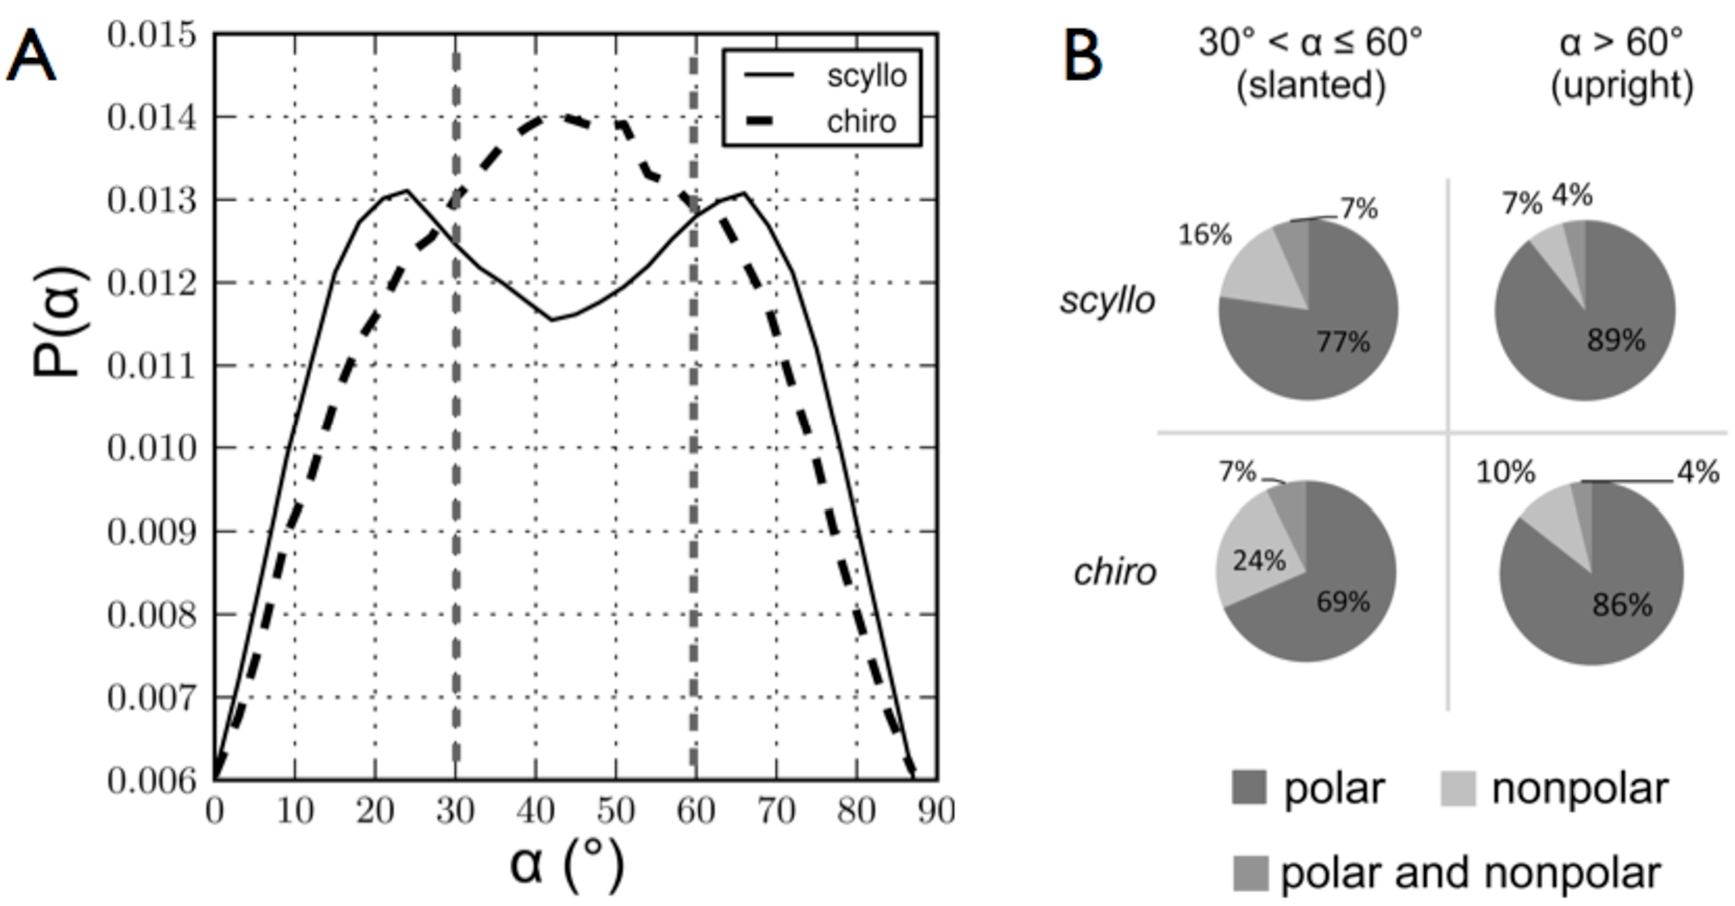
\includegraphics[width=6in]{figures/results1/GA4_paper_figures_submitted-8-rearranged}
  \caption[Binding mode and orientation of \textit{scyllo-} and \textit{chiro-}inositol to the fibril of \gafour.]{Binding mode and orientation of \textit{scyllo-} and \textit{chiro-}inositol to the fibril of \gafour. The distribution of inositol to sheet planar angles is depicted in A). B) Inositol binding to nonpolar and polar groups as classified by $\alpha$, the angle at which inositol molecules bind at the surface of the fibrillar \gafour\ (see Methods).}
   \label{fig:figure8}
\end{figure}

\section{Discussion}
In the above analysis, we have systematically characterized the association of stereoisomers \textit{scyllo-}, \textit{epi-}, \textit{myo-} and \textit{chiro-}inositol with alanine dipeptide, a simple model of the peptidic backbone. Furthermore, we examined the binding of \textit{scyllo-} and \textit{chiro-}inositol to various aggregated states of \gafour\ to probe the role of backbone binding in amyloid inhibition. Our results show that inositol exhibits weak binding with dissociation constants in the range of 0.04 M to 1 M to the different peptides and aggregation states considered.

Furthermore, the \KD\ of inositol increases linearly with the number of peptide groups in the system (Table~\ref{tab:binding_constants}), indicating that inositol does not bind cooperatively to the monomer and aggregate states of \gafour\ considered. As expected, inositol binds most weakly to alanine dipeptide, with a value about 4 times smaller than the \KD\ of urea to N-acetyl alanine reported recently in the literature (0.3 M for urea\cite{Lee:2010p59} vs 1.1 M for \textit{scyllo-}inositol). Taken together, our results indicate that the activity of inositol stereoisomers is similar to that of osmolytes, which typically have binding constants in the millimolar to molar range.\cite{Rosgen:2007p90,Street:2006p21}

Moreover, our results are consistent with the hypothesis that osmolytes influence protein and peptide folding and stability through direct binding rather than by modifying solvent properties.\cite{Canchi:2011p53,Lee:2010p59,Street:2006p21} The spacing of consecutive OH groups of inositol is well-suited to bidentate interactions with adjacent groups of the polypeptide backbone (Figure~\ref{fig:figure2}A). Our findings shown in Figure~\ref{fig:figure2}A are consistent with similar binding modes observed in a recent ab initio simulation and IR spectroscopic study of the binding of glucose epimers to the phenylalanine dipeptide backbone.\cite{Cocinero:2011p54} Furthermore, inositol stereoisomers displace the backbone conformation of alanine dipeptide towards extended $\beta$-strand conformations (Figure~\ref{fig:figure2}B). However, neither \textit{scyllo-} nor \textit{chiro-}inositol had a significant effect on the conformational equilibrium of the \gafour\ monomer. Taken together, these results indicate that inositol may not act as a drug by directly influencing monomer conformations. However, our results do not preclude the possibility that inositol may block fibril elongation by preferentially binding to monomers that are constrained to extended conformations, such as those at exposed edges of \bsheets.

Independently of the presence of inositol, both the preformed \bsheet\ oligomer and the monodisperse solution of \gafour\ evolved into a similar morphology (Figure~\ref{fig:figure4}B and \ref{fig:figure5}) with only a small amount of $\beta$-structure (Figure~\ref{fig:figure4}B), indicating that small aggregates of \gafour\ are likely to be disordered. Unlike the hydrophobic core of the \abeta\ peptide, \gafour\ is a shorter and more polar peptide that is capable of forming more hydrogen bonds than nonpolar contacts. Our results show that peptide-peptide hydrogen bonding play an important role in the aggregation of \gafour\ peptides in solution (Figure~\ref{fig:figure5}). Because neither stereoisomer disrupted the aggregates of \gafour, our results indicate that inositol is unlikely to inhibit fibril formation by breaking up preformed aggregates. Therefore, we conclude that inositol is unlikely to inhibit fibril formation by binding monomers and small disordered oligomers since binding appears to be weak, non-cooperative, and stereochemistry-independent.

By contrast, although the dissociation constants were similar for both \textit{scyllo-} and \textit{chiro-}inositol, binding specificity and binding modes involving nonpolar groups of the fibrillar aggregate of \gafour\ were modulated by the stereochemistry of inositol. A significantly higher fraction of \textit{chiro-}inositol than \textit{scyllo-}inositol was bound to nonpolar groups of the fibrillar aggregate (Figure~\ref{fig:figure6}E). Moreover, \textit{scyllo-}inositol exhibited a bimodal distribution of binding orientations, with a significant preference for orientations in which the ring of inositol is either parallel or perpendicular to the mean surface of the \bsheet\ over \textit{chiro-}inositol (Figure~\ref{fig:figure7}). As a direct consequence of the presence of axial hydroxyl groups, \textit{chiro-}inositol is more likely to bind at angles that promote contact with nonpolar groups at the surface of the fibrillar aggregate, whereas the more specific binding modes of \textit{scyllo-}inositol favors backbone binding. Since this is the only stereochemistry-dependent result of our study, we speculate that \textit{scyllo-}inositol acts on ordered \bsheet\ aggregates (as opposed to disordered oligomers or monomers). Moreover, these findings suggest a possible mechanism of action whereby a significant binding affinity to specific side chains on the surface of fibrillar aggregates could lead to the inhibition of \bsheet\ stacking (and therefore, amyloid fibril growth or maturation) by \textit{scyllo-}inositol. Similarly, different binding modes observed in MD simulations of \abeta42 fibrils have been proposed to explain differences in binding affinities between Thioflavin T, a well-known amyloid-binding dye, and its chemical analogs.\cite{Mathis:2003p55,Wu:2011p24}

A factor that we have not considered in this study is the influence of inositol:peptide molar ratio on binding and inhibition. In vitro, the inhibition activity of \textit{scyllo-}inositol was observed at an inositol:peptide ratio of 25:1, where inositol stereoisomers were present in excess of \abeta\ at concentrations of 0.25 mM to 5 mM.\cite{McLaurin:2000p64} Although our simulations had effective concentration of inositol an order of magnitude higher than in these experiments, it is possible that we have precluded cooperative inositol binding modes by limiting the number of inositol molecules present in the small simulation cell. Furthermore, \KD\ values obtained from our simulations of \gafour\ were approximately two orders of magnitude higher than measured for \abeta. Based on our results, the predicted \KD\ of (GA)$_{21}$, a Gly-Ala repeat peptide similar in length to \abeta, would be 1200 mM/21 = 57 mM, which is still an order of magnitude greater than \textit{in vitro} inhibitory concentrations. This indicates that \textit{scyllo-}inositol is unlikely to inhibit \bsheet\ formation by \gafour\ peptides, and more importantly, that backbone binding by small molecules may not be sufficient for inhibition of amyloid formation. In future studies, elucidating the relationship of binding cooperativity and amyloid inhibition by approaching experimental drug:protein molar ratios, as well as elucidating the sequence specificity of inositol binding to amyloid fibrils, will provide further insight that may be used in the rational drug design of improved inhibitors.

\section{Conclusions}
We have performed systematic simulations of simple amyloidogenic peptide models with both active and inactive stereoisomers of inositol to examine the molecular basis of amyloid inhibition. Our results indicate that although peptide backbone dominates the interaction with inositol, the binding affinity is low and remains in the millimolar range. Moreover, this property is independent of stereochemistry and does not appear to be sufficient to impede peptide dimerization through intermolecular backbone hydrogen bonding. Taken together, our results suggest that amyloid inhibition by inositol cannot be accounted for by generic binding to the peptidic backbone alone and is likely to involve sequence-specific interactions with amino-acid side chains as well as binding to specific aggregate morphologies. Accordingly, although the formation of intermolecular hydrogen bonds is the predominant interaction in protein aggregates composed of \gafour, amyloidogenic peptides involved in amyloid diseases are often more hydrophobic and in general, self-aggregation is driven largely by the hydrophobic effect.\cite{Chiti:2006p20} In forthcoming studies, we will examine the role of sequence-specific interactions between inositol and aggregates of pathogenic peptides.

\section*{Acknowledgements}
This work was made possible by the Centre for Computational Biology at the Hospital for Sick Children, the facilities of the Shared Hierarachical Academic Research Computing Network(SHARCNET, www.sharcnet.ca), the GPC supercomputer at the SciNet HPC Consortium and Compute/Calcul Canada. This work was supported in parts by a fellowship from the Heart and Stroke Foundation of Ontario, a Canada Graduate Scholarship from the National Science and Engineering Research Council, the Research Training Center at the Hospital for Sick Children, and the Canadian Institutes of Health Research (Grant No. MOP84496). R.P. is a CRCP chairholder.

\begin{singlespace}
\addcontentsline{toc}{section}{Bibliography}
\bibliographystyle{elsart-num}
\bibliography{results1/results1}
\end{singlespace}
